\documentclass{article}
\usepackage{amsmath, amssymb, amsfonts}
\usepackage{tikz}
\usetikzlibrary{decorations.pathmorphing}

\newcommand{\op}{\prime}
\title{Crystals of Inert Elements}
\begin{document}
\author{Amey Joshi}
\maketitle
Elements of group VIII are inert gases. They solidify at low temperature and
high pressure. The electronic configuration of atoms of these elements in 
crystalline form is not drastically different from gas phase. The binding of
the crystals is not because of an overlap of electronic orbitals. It is due to
a rather weak interaction arising due to dipole moments in atoms. If the charge
configuration of atoms is static then a neutral atom will have zero electric
field in its exterior. However, the charge distribution of an atom flucuates,
resulting in a dipole moment. A dipole moment of one atom results in the 
polarisation of its neighbouring atoms, which in turn polarise their neighbours
and soon all atoms in a crystal are polarised. 

We will model the atomic dipole moment as a pair of opposite charges connected
by a an ideal spring.
\begin{figure}[htbp]
  \centering
  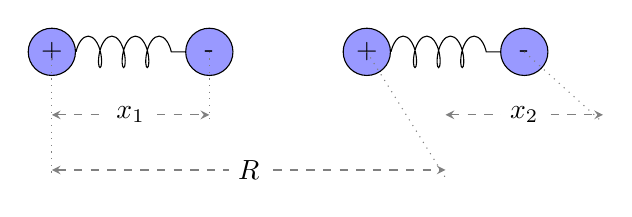
\begin{tikzpicture}[
    % Define a style for the atoms
    atom/.style={circle, draw=black, fill=blue!40, minimum size=6mm, inner sep=0pt},
    % Define a style for the springs
    spring/.style={decorate, decoration={coil, aspect=0.4, segment length=3mm, amplitude=2mm}},
    dimline/.style={<->, >=stealth, thin, dashed, gray}
  ]

    % Place the 4 atoms in a row
    \node[atom] (A1) at (0,0) {+};
    \node[atom] (A2) at (2,0) {-};
    \node[atom] (A3) at (4,0) {+};
    \node[atom] (A4) at (6,0) {-};

    % Connect Atom 1 and Atom 2 with a spring
    \draw[spring] (A1) -- (A2);

    % Connect Atom 3 and Atom 4 with a spring
    \draw[spring] (A3) -- (A4);

     % --- DISTANCE MEASUREMENTS (BELOW THE ATOMS) ---

    % Distance x1: Between A1 and A2
    \draw[dimline] (0,-0.8) -- (2,-0.8)
      node[midway, fill=white, text=black] {$x_1$};

    % Distance x2: Between A3 and A4
    \draw[dimline] (5,-0.8) -- (7,-0.8)
      node[midway, fill=white, text=black] {$x_2$};

    % Distance R: Center-to-center between A1 and A3
    \draw[dimline] (0,-1.5) -- (5,-1.5)
      node[midway, fill=white, text=black] {$R$};

    % Optional: Subtle guide lines connecting atoms to the measurement arrows
    \draw[dotted, gray] (A1.center) -- (0,-1.6);
    \draw[dotted, gray] (A2.center) -- (2,-0.9);
    \draw[dotted, gray] (A3.center) -- (5,-1.6);
    \draw[dotted, gray] (A4.center) -- (7,-0.9);

  \end{tikzpicture}
  \caption{A model of two polarised inert element atoms.}
  \label{f1}
\end{figure}
The hamiltonian of each atom can be written as 
\[
\frac{p^2}{2m} + \frac{1}{2}Cx^2,
\]
where $x$ is the distance between the two charges, $p$ is their reduced momentum
and $m$ their reduced mass. (Section \ref{s2} explains how to convert the 
two-body problem into two one-body problems using standard techniques from
classical mechanics.) The hamiltonian of two atoms ignoring the 
interaction between them is
\begin{equation}\label{e1}
H_0 = \frac{p_1^2}{2m}+\frac{1}{2}Cx_1^2+\frac{p_2^2}{2m}+\frac{1}{2}Cx_2^2
\end{equation}
Assume that each charge has an equal magnitude, say $q$, the electrostatic
interaction can be represented by the perturbation
\begin{equation}\label{e2}
H_1 = \frac{q^2}{R} - \frac{q^2}{R + x_2} - \frac{q^2}{R - x_1} + 
\frac{q^2}{R + x_2 - x_1}.
\end{equation}
If $R \gg x_1, x_2$, we can use the generalised binomial expansion
\begin{equation}\label{e3}
(1 - x)^\alpha = 1 - \alpha x + \frac{1}{2!}\alpha(\alpha - 1)x^2 - 
\frac{1}{3!}\alpha(\alpha - 1)(\alpha - 2)x^3 + \cdots
\end{equation}
to get
\begin{equation}\label{e4}
H_1 = -\frac{2qx_1x_2}{R^3}.
\end{equation}
The total hamiltonian of the system is
\begin{equation}\label{e5}
H = \frac{p_1^2}{2m}+\frac{1}{2}Cx_1^2+\frac{p_2^2}{2m}+\frac{1}{2}Cx_2^2
- \frac{2qx_1x_2}{R^3}.
\end{equation}
Introduce the coordinates
\begin{eqnarray}
x_s &=& \frac{1}{\sqrt{2}}(x_1 + x_2) \label{e6} \\
x_a &=& \frac{1}{\sqrt{2}}(x_1 - x_2) \label{e7}
\end{eqnarray}
where the subscripts stand for symmetric and anti-symmetric combinations of
the original coordinates. In terms of these, the total hamiltonian is
\begin{equation}\label{e8}
H = \frac{p_1^2}{2m} + \frac{p_2^2}{2m} + \frac{1}{2}\left(C - \frac{2e^2}{R^3}
\right)x_s^2 + \frac{1}{2}\left(C + \frac{2e^2}{R^3}\right)x_a^2
\end{equation}
This is the hamiltonian of two uncoupled oscillators of spring constants
\[
C \pm \frac{2e^2}{R^3}.
\]
The fundamental frequencies of these oscillators are
\begin{eqnarray}
\omega_s &=& \omega_0\sqrt{1 - \frac{2e^2}{CR^3}} \label{e9} \\
\omega_a &=& \omega_0\sqrt{1 + \frac{2e^2}{CR^3}} \label{e10}
\end{eqnarray}
where $\omega_0 = \sqrt{C/m}$ is the frequency of the original, uncoupled
oscillators. The ground state energy of these oscillators is
\begin{equation}\label{e11}
U = \hbar\omega_s + \hbar\omega_a = \hbar\omega_0\left(1 - \frac{1}{2}\left(
\frac{e^2}{CR^3}\right)^2\right)
\end{equation}
As compared to the total energy $\hbar\omega_0$ of the two uncoupled
oscillators, the dipole-dipole coupling results in a reduction in energy by 
\begin{equation}\label{e12}
\delta U = -\frac{1}{2}\hbar\omega_0\left(\frac{e^2}{CR^3}\right)^2
= -\frac{A}{R^6},
\end{equation}
where $A > 0$ is a constant dependent on the molecular properties.

A potential of form of \eqref{e12} results in an attractive force between the
two atoms. However, the atoms cannot come arbitrarily close to each other. When
they attempt to do so, their electronic orbitals being to overlap and because
they are completely filled, Pauli's exclusion principle prevents them from
getting any closer. It is experimentally found that this repulsive potential can
be expressed as $B/R^{12}$ for a positive constant $B$.

Thus the net interaction between two inert element atoms can be represented by
\begin{equation}\label{e13}
U(r) = -4\varepsilon\left[\left(\frac{\sigma}{r}\right)^6 - 
\left(\frac{\sigma}{r}\right)^{12}\right],
\end{equation}
where $\sigma$ and $\varepsilon$ are constants. It is also called the Lennard-
Jones potential.

Now suppose there is a crystal of $N$ atoms bound by Van der Waals force. The
total potential energy is a sum of terms \eqref{e13} for each pair of atoms.
Thus,
\begin{equation}\label{e14}
U_{\text{tot}} = -2\varepsilon\left[
\sum_{i \ne j}\left(\frac{\sigma}{r_{ij}}\right)^6 - 
\sum_{i \ne j}\left(\frac{\sigma}{r_{ij}}\right)^{12}\right]
\end{equation}
If we ignore the surface effects, each atom contributes equally to $U_{tot}$.
Under this approximation, we can write \eqref{e14} as
\begin{equation}\label{e15}
U_{\text{tot}} = -2\varepsilon N\left[
\sum_{i \ne j}\left(\frac{\sigma}{r_{ij}}\right)^6 - 
\sum_{i \ne j}\left(\frac{\sigma}{r_{ij}}\right)^{12}\right]
\end{equation}
where the term in square brackets is for an arbitrarily chosen $i$-th atom in
the bulk of the crystal. If $R$ is the nearest neighbour distance, it one can
express $r_{ij} = Rp_{ij}$ and write \eqref{e15} as
\begin{equation}\label{e16}
U_{\text{tot}} = -2\varepsilon N\left[
\frac{\sigma^6}{R^6}\sum_{i \ne j}\frac{1}{p_{ij}^6} - 
\frac{\sigma^{12}}{R^{12}}\sum_{i \ne j}\frac{1}{p_{ij}^{12}}\right].
\end{equation}

Examples of inert element crystals:
\begin{enumerate}
\item Helium solidifies as hcp crystal. The sums in \eqref{e16} evaluate to
\[
\sum_{i \ne j}\frac{1}{p_{ij}^6} = 14.15489, \;
\sum_{i \ne j}\frac{1}{p_{ij}^{12}} = 12.13229.
\]

\item Neon, Argon, Krypton, Xenon and Radon solidify as fcc crystal. For these
crystals, the sums evaluate to
\[
\sum_{i \ne j}\frac{1}{p_{ij}^6} = 14.45382, \;
\sum_{i \ne j}\frac{1}{p_{ij}^{12}} = 12.13188.
\]

\item Neon can also form bcc crystals for which
\[
\sum_{i \ne j}\frac{1}{p_{ij}^6} = 12.2533, \;
\sum_{i \ne j}\frac{1}{p_{ij}^{12}} = 9.11418
\]
\end{enumerate}

To make the notation less cluttered, we denote the sum as
\begin{equation}\label{e17}
\sum_{i \ne j}\frac{1}{p_{ij}^6} = P, \;
\sum_{i \ne j}\frac{1}{p_{ij}^{12}} = Q
\end{equation}
so that \eqref{e16} is
\[
U_{\text{tot}} = -2\varepsilon N\left(\frac{P\sigma^6}{R^6} - \frac{Q\sigma^12}
{R^{12}}\right).
\]
The equilibrium value of $R$ is the one that minimises $U_\text{tot}$. As
\[
\frac{dU_{\text{tot}}}{dR} = -2\varepsilon N\left(-\frac{6P\sigma^6}{R^7} +
\frac{12Q\sigma^{12}}{R^{13}}\right).
\]
the function $U_\text{tot}$ has an extremum when
\begin{equation}\label{e18}
\frac{6P\sigma^6}{R^7} = \frac{12Q\sigma^{12}}{R^{13}} \Rightarrow
\frac{6P\sigma^7}{R^7} = \frac{12Q\sigma^{13}}{R^{13}} \Rightarrow
\frac{R}{\sigma} = \left(\frac{2Q}{P}\right)^{1/6}.
\end{equation}

The equilibrium cohesive energy for these crystals is evaluated by substituting
the $R/\sigma$ found in \eqref{e18} into \eqref{e16}.


\section{Two masses connected by a spring}\label{s2}
Consider two masses $m_1$ and $m_2$ connected by an ideal spring as shown
in the figure. Let the origin be at the centre of the spring when the spring
is in its relaxed state. The equations of motion of the two masses are
\begin{eqnarray}
m_1\ddot{x}_1 &=& F_1^e + F_{21} \label{s2e1} \\
 m_2\ddot{x}_2 &=& F_2^e + F_{12} \label{s2e2}
\end{eqnarray}
where $F_1^e$ and $F_2^e$ are the external forces on the masses, $F_{21}$ is
the force of mass $m_2$ on $m_1$ and $F_{12}$ is its reaction. 

\begin{figure}[htbp]
  \centering
  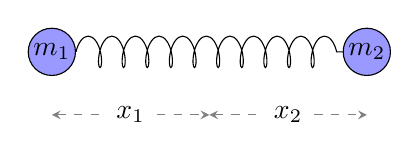
\begin{tikzpicture}[
    % Define a style for the atoms
    atom/.style={circle, draw=black, fill=blue!40, minimum size=6mm, inner sep=0pt},
    % Define a style for the springs
    spring/.style={decorate, decoration={coil, aspect=0.4, segment length=3mm, amplitude=2mm}},
    dimline/.style={<->, >=stealth, thin, dashed, gray}
  ]

    % Place the 4 atoms in a row
    \node[atom] (A1) at (0,0) {$m_1$};
    \node[atom] (A2) at (4,0) {$m_2$};

    % Connect Atom 1 and Atom 2 with a spring
    \draw[spring] (A1) -- (A2);

     % --- DISTANCE MEASUREMENTS (BELOW THE ATOMS) ---

    % Distance x1: Between A1 and A2
    \draw[dimline] (0,-0.8) -- (2,-0.8)
      node[midway, fill=white, text=black] {$x_1$};

    % Distance x2: Between A3 and A4
    \draw[dimline] (2,-0.8) -- (4,-0.8)
      node[midway, fill=white, text=black] {$x_2$};

  \end{tikzpicture}
  \caption{Two masses connected by an ideal spring.}
  \label{f2}
\end{figure}

Introduce the coordinates
\begin{eqnarray}
X &=& \frac{m_1x_1 + m_2x_2}{m_1 + m_2} \label{s2e3} \\
x &=& x_2 - x_1 \label{s2e4}
\end{eqnarray}
Adding \eqref{s2e1} and \eqref{s2e2} gives $M\ddot{X} = F_1^e + F_2^e = F^e$,
the total external force. Subtracting \eqref{s2e1} from \eqref{s2e2} gives
\[
\frac{m_1m_2}{m_1 + m_2}\ddot{x} = F_{21}.
\]
We define the reduced mass of the system as
\begin{equation}\label{s2e5}
\frac{1}{m} = \frac{1}{m_1} + \frac{1}{m_2}
\end{equation}
so that we get 
\begin{equation}\label{s2e6}
m\ddot{x} = F_{21},
\end{equation}
as the second equation of motion. Since $F_{21}$ is a force due to the spring,
we have $m\ddot{x} = -Cx$ as the equation of motion of the reduced mass. Note
that $x$ is the distance between the two masses.
\end{document}
